\newpage
\section{Multivibratore astabile}
Si è montato il circuito in \fig{astab_sch}, con i seguenti valori dei componenti:

\begin{figure}[H]
	\begin{minipage}{0.8\textwidth}
		\centering
		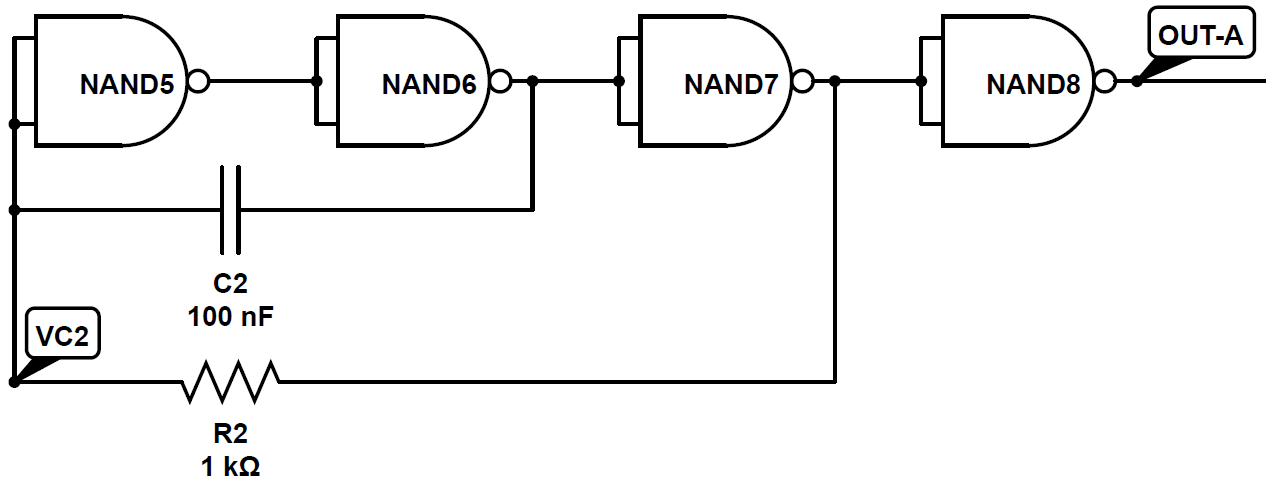
\includegraphics[scale=0.35]{astabile.png}
		\caption{Multivibratore astabile}
		\label{astab_sch}
	\end{minipage}
	\begin{minipage}{0.1\textwidth}
		\begin{tabular}{l}
			$R_2 = \SI{982(8)}{\ohm}$\\
			$C_2 = \SI{109(4)}{\nano \farad}$
		\end{tabular}
	\end{minipage}
\end{figure}

Si è verificato che il segnale in uscita fosse un onda quadra, come visibile in \fig{astab_osc} e si sono misurati periodo è duty cycle, che risultano valere:
$$T = \SI{204(1)}{\micro \second} \qquad D\% = \SI{70.1(6)}{\%}$$

\begin{figure}[H]
	\centering
	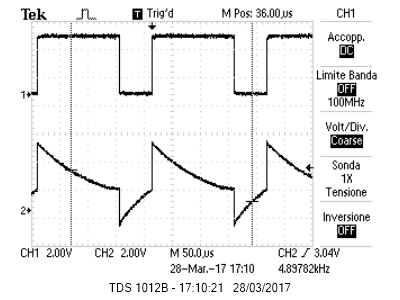
\includegraphics[scale=1]{astabile_inout.png}
	\caption{OUT-A e VC2 del multivibratore astabile}
	\label{astab_osc}
\end{figure}

Si è quindi andati ad osservare la forma d'onda all'ingresso del primo NAND (VC2), come visibile nella stessa \fig{astab_osc}.
La tensione oscilla tra \SI{4.48(12)}{\volt} e \SI{-0.68(2)}{\volt}, mentre la commutazione avviene a \SI{1.44(4)}{\volt}.

\subsection{Analisi del funzionamento}

Per spiegare il comportamento del circuito facciamo riferimento alla \fig{astab_expl}.
Consideriamo un istante prima della commutazione basso/alto del NAND6 (o equivalentemente sull'uscita OUT-A): VC2 si appresta a superare $V_{comm}=\SI{1.44}{\volt}$ (la tensione di commutazione) e, essendo l'uscita del NAND6 bassa, la tensione sul condensatore è proprio uguale a VC2 ($\Delta V_C = VC_2 - V_{NAND6}$).

Raggiunta la tensione di commutazione l'uscita del NAND6 viene forzata allo stato HIGH e l'uscita del NAND7 si troverà in stato LOW, questo aumenterà istantaneamente la tensione VC2 di $V_{HIGH}=\sim \SI{3.04}{\volt}$, pari alla tensione dello stato HIGH della porta logica. Da questo punto in poi il condensatore si scaricherà con un $\tau = RC$, fino a raggiungere nuovamente la tensione di commutazione.

Nel passaggio alto/basso del NAND6 la situazione è diversa: VC2 dal valore di $\sim \SI{1.44}{\volt}$ non può diminuire oltre i $\sim\SI{-0.7}{\volt}$ per la presenza di diodi di protezione agli ingressi delle porte logiche, a questo è dovuta l'asimmetria dei semiperiodi.

\begin{figure}[H]
	\centering
	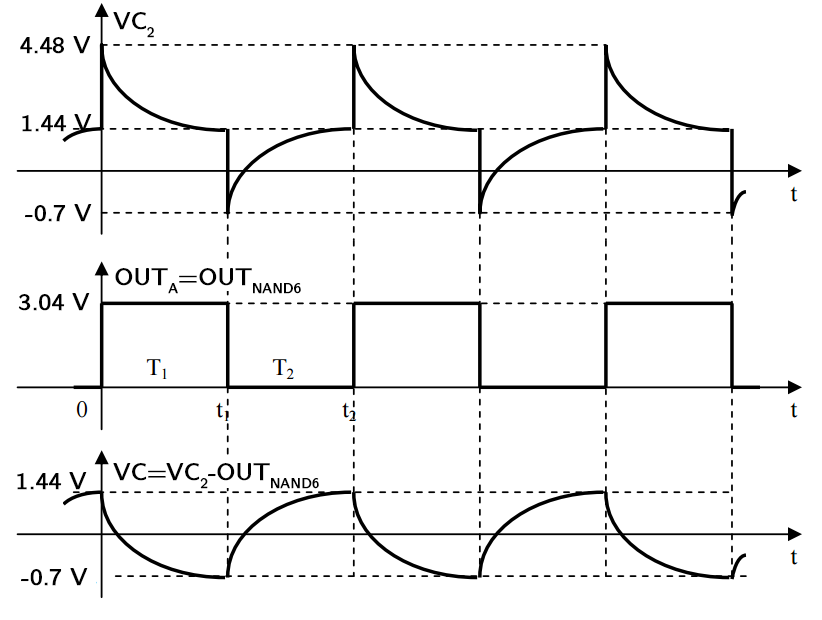
\includegraphics[scale=0.3]{astab_graph.png}
	\caption{forme d'onda nei vari punti del circuito}
	\label{astab_expl}
\end{figure}

Il semiperiodo HIGH è atteso essere pari a $RC\times \ln(V_{HIGH}/V_{comm}) = \SI{122(5)}{\micro\second}$, non compatibile con quello misurato di \SI{143(1)}{\micro\second}, il motivo è da ricercarsi probabilmente nel fatto che, diversamente da come schematizzata in \fig{astab_expl}, l'uscita del NAND6 non appariva costante ma aumentava leggermente nel corso del semiperiodo.
	
\subsection{Linearità del periodo con la resistenza}
Si è variata la resistenza $R_2$ in un intorno di $\SI{1000}{\ohm}$ e per ogni valore di resistenza di è misurato il periodo del segnale. I risultati raccolti sono riportati in appendice in \tab{astab_data}.
Si è quindi proceduto ad un fit lineare ($ax+b$), ottenendo i seguenti risultati:
$$a = \SI{20.74(27)}{\ohm / \micro\second} \qquad b=\SI{1.6 \pm 2.5}{\micro \second} \qquad \chi^2/ndof = 10.7/7 \qquad corr(a,b)= -0.966$$
In \fig{astab_lin} sono rappresentati i dati raccolti e il fit eseguito.

\begin{figure}[h!]
	\centering
	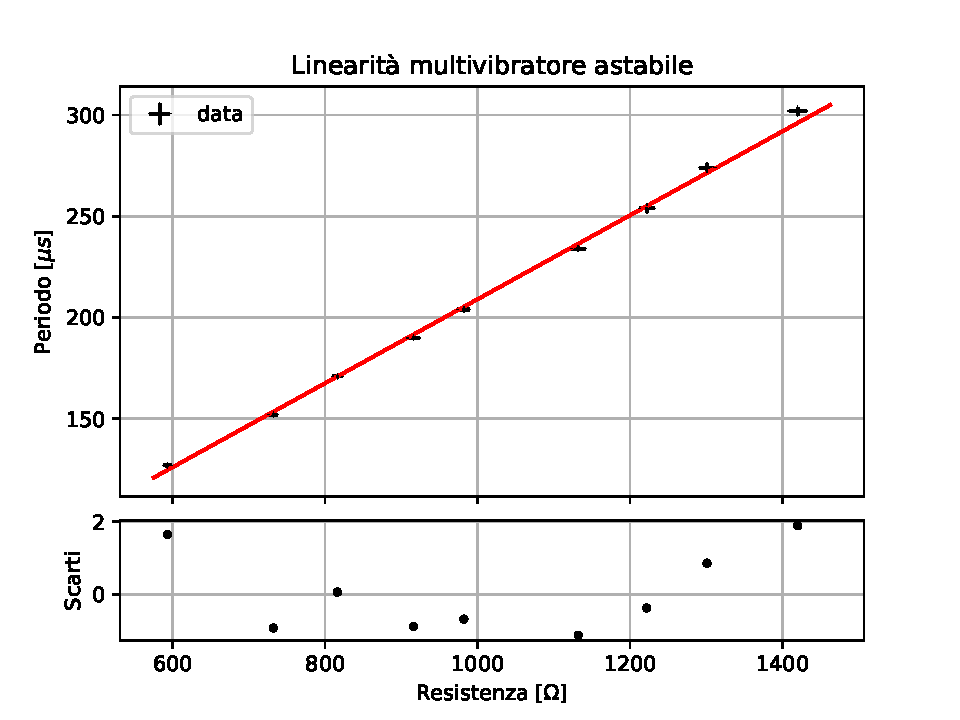
\includegraphics[scale=0.9]{fit_dati_3.pdf}
	\caption{Dati raccolti e fit della linearità del multivibratore astabile}
	\label{astab_lin}
\end{figure}



